\documentclass[11pt]{article}

\usepackage[margin=1in]{geometry}
\usepackage{color,url,graphicx,colortbl, amsmath, amsfonts}
\usepackage{multirow,amsthm}
\usepackage{float,framed,xspace}
\usepackage{times, microtype}
\usepackage{enumitem}
\usepackage{hyperref}

\usepackage{listings}
\definecolor{dkgreen}{rgb}{0,0.6,0}
\definecolor{gray}{rgb}{0.5,0.5,0.5}
\definecolor{mauve}{rgb}{0.58,0,0.82}

\usepackage{courier}
\lstset{
  basicstyle=\footnotesize\ttfamily, % Standardschrift
  %numbers=left,               % Ort der Zeilennummern
  numberstyle=\tiny,          % Stil der Zeilennummern
  %stepnumber=2,               % Abstand zwischen den Zeilennummern
  numbersep=5pt,              % Abstand der Nummern zum Text
  tabsize=2,                  % Groesse von Tabs
  extendedchars=true,         %
  breaklines=true,            % Zeilen werden Umgebrochen
  keywordstyle=\color{blue},
  % frame=b,         
  %        keywordstyle=[1]\textbf,    % Stil der Keywords
  %        keywordstyle=[2]\textbf,    %
  %        keywordstyle=[3]\textbf,    %
  %        keywordstyle=[4]\textbf,   \sqrt{\sqrt{}} %
  stringstyle=\color{mauve}\ttfamily, % Farbe der String
  showspaces=false,           % Leerzeichen anzeigen ?
  showtabs=false,             % Tabs anzeigen ?
  xleftmargin=17pt,
  framexleftmargin=17pt,
  framexrightmargin=5pt,
  framexbottommargin=4pt,
  %backgroundcolor=\color{lightgray},
  showstringspaces=false      % Leerzeichen in Strings anzeigen ?        
}
\lstloadlanguages{% Check Dokumentation for further languages ...
  %[Visual]Basic
  %Pascal
  C
  %C++
  %XML
  %HTML
  %Java
 }

\newcommand{\URL}[1]{\url{#1}}

\hyphenation{App-Engine php-BB}
\renewcommand{\ttdefault}{pxtt}
\newcommand{\name}{OPS\@\xspace}

\begin{document}

\title{Query rewriting notes}
 %\author{Raluca Ada Popa and Nickolai Zeldovich  \\
 %      {\em MIT CSAIL}}
\date{}

\newcommand{\Z}{\mathbb{Z}}
\newcommand{\gf}{\mathrm{GF}}
\newcommand{\F}{\mathbb{F}}
\newcommand{\G}{\mathbb{G}}

\newcommand{\enc}{\mathsf{Enc}}
\newcommand{\paramsgen}{\mathsf{ParamsGen}}
\newcommand{\keygen}{\mathsf{KeyGen}}
\newcommand{\curvegen}{\mathsf{CurveGen}}
\newcommand{\adj}{\mathsf{Adj}}
\newcommand{\tok}{\mathsf{Token}}
\newcommand{\prp}{\mathsf{PRP}}
\newcommand{\adjprp}{\textsf{ADJ-PRP}}
\newcommand{\aprp}{\textsf{AdjPRP}}


% requires amsthm, enumitem
\theoremstyle{algorithms}
\newtheorem{construction}{Algorithm}
\newcommand{\ALGORITHM}[4]{%  name, llabel, intro, \items
  \begin{construction}[#1]\label{#2} \mbox{}
  \normalfont\noindent
  #3
  \vspace{0.13\baselineskip}
  \begin{enumerate}[noitemsep,nolistsep]\itemsep=0.1\baselineskip 
  #4
  \end{enumerate}
  \end{construction}
}


\renewcommand{\qed}{\hfill \ensuremath{\Box}}



\newcommand{\sk}{\mathsf{sk}}
\newcommand{\SK}{\mathsf{SK}}
\newcommand{\params}{\mathsf{params}}


\newcommand{\skcol}{\sk_{\mathsf{col}}}
\newcommand{\skmsg}{\sk_{\mathsf{msg}}}


\newcommand{\csk}{\mathsf{csk}}
\newcommand{\omsg}{\mathsf{O}^k_{\mathsf{msg}}}
\newcommand{\ocol}{\mathsf{O}^k_{\mathsf{col}}} 
\newcommand{\chb}{\mathsf{Ch}^{\mathsf{B}}}
\newcommand{\sch}{\mathsf{SCh}}
\newcommand{\calk}{\mathcal{K}}

\newcommand{\negl}{\mathsf{negl}}

\newcommand{\la}{\leftarrow}
\newcommand{\ra}{\rightarrow}

\newcommand{\cald}{\mathcal{D}}

\newcommand{\RND}{\textrm{RND\@}}
\newcommand{\DET}{\textrm{DET\@}}
\newcommand{\OPE}{\textrm{OPE\@}}
\newcommand{\OPEJOIN}{\textrm{OPE-JOIN\@}}
\newcommand{\HOM}{\textrm{HOM\@}}
\newcommand{\JOIN}{\textrm{JOIN\@}}
\newcommand{\SEARCH}{\textrm{SEARCH\@}}
\newcommand{\HIGH}{\textrm{HIGH\@}}
\newcommand{\minenc}{\textrm{MinEnc}}

\newcommand{\adjjoin}{\textsf{ADJ-JOIN}}

\newcommand{\rap}[1]{\textcolor{blue}{RAP: #1}}
\newcommand{\nz}[1]{\textcolor{red}{NZ: #1}}
\newcommand{\todo}[1]{\noindent{\small \textcolor{blue}{Todo: #1}}}
\newcommand{\draft}[1]{\textcolor{red}{#1}}



\newcommand{\adv}{\mathsf{Adv}}
\newcommand{\ch}{\mathsf{Ch}}


\newtheorem{definition}{Definition}
\newtheorem{theorem}{Theorem}
\newtheorem{remark}{Remark}
\newtheorem{lemma}[theorem]{Lemma}
\newtheorem{corollary}[theorem]{Corollary}
\newtheorem{proposition}[theorem]{Proposition}
\newtheorem{claim}[theorem]{Claim}
\newtheorem{observation}{Observation}


\maketitle

This note is a brief description of the query rewriting algorithm of
CryptDB~\cite{PopaRZB11:CryptDB}. 



A query is first parsed into a lex tree using the MySQL parser, and then it is
rewritten. The unit in a lex tree is a SQL item, which can be a field, a constant,
an operations, or even an expression.
Query rewriting from a lex tree happens in two phases:
\begin{enumerate}
  \item Gather: gathers information about all the possible ways an item could be
    rewritten to support the operations in the query.
  \item Rewrite: Based on the information gathered, rewrite encrypts constants,
    replaces fields with the names of their onions, and rewrites some operations
    into new operations or in UDFs.
\end{enumerate}

We defined a class for each type of field, constant, or operation, that is meant
to handle gather (\texttt{do\_gather\_type}) and rewrite
(\texttt{do\_rewrite\_type}) for this type of item. 


\section{Gather}

\begin{lstlisting}
virtual EncSet do_gather_type(Item_field *i, reason &tr, Analysis & a) const;
\end{lstlisting}

Before defining EncSets, let us define \textit{OLK}, which stands for (onion, security
level, key). This is all the information one needs to encrypt or rewrite an
item. The key is a pointer to the metadata of a field (FieldMeta) because each field has
its own key in CryptDB. The key is not stored in FieldMeta directly, but rather
it is stored as a list of EncLayers, which implement encryption or decryption with
this key given a value.

An \textit{EncSet} is ``a set of possible encryption types of an item''. That
is, a set of OLKs with which an item could be encrypted or rewritten. Instead of
listing all the OLKs in an EncSet, the EncSet rather contains a map of onions to
the highermost security level and a key, with the understanding that all lower levels on
the same onions are also in the EncSet.

\texttt{do\_gather\_type} returns an \textit{outgoing} EncSet, which consists of all the
different OLKs with which item i could be encrypted/rewritten.

\texttt{reason} indicates the reason why such an outgoing EncSet was returned,
and it is useful for printing out detailed error messages when some operation
cannot be supported.

We now describe how \texttt{do\_gather\_type} works. It traverses the lex
structure bottom up. Consider the case that $i$ is a leaf node. If $i$ is a field, it returns the
encset that $i$ can support (``PLAIN'' if the field is not encrypted). If $i$ is
a constant, it returns ``all enc layers with
      any key and PLAIN''

\newcommand{\es}{\mathsf{EncSet}}

Let's present a generic gather for an operation. 

\ALGORITHM{Gather at item $i$}{alg:gather}{}{
    \item Run gather on each child of $i$. Let $\es_j$ be the encset returned from
    each child.
    \item Consider the encryption levels needed to perform the operation of $i$,
      \textit{needed EncSet}. Based on the child encsets $\es_j$ and the needed EncSet,
      find solutions: sets of OLKs that could be
      used for each child and the computation at $i$ to support the operation at
      $i$.
      \begin{enumerate}
      \item If the set is null, throw unsupported query error and use the
        information at this node and the 
      \texttt{reason}s from the children to explain why.
      \item If there
      are solutions, store them in a RewritePlan to be used during
      rewrite. Compute the resulting OLKs for each possible solution, and
      aggregate them in the outgoing EncSet, to be returned.
      \end{enumerate}
}

Figure~\ref{fig:gather} provides an example.

\begin{figure}[t!]
\centering
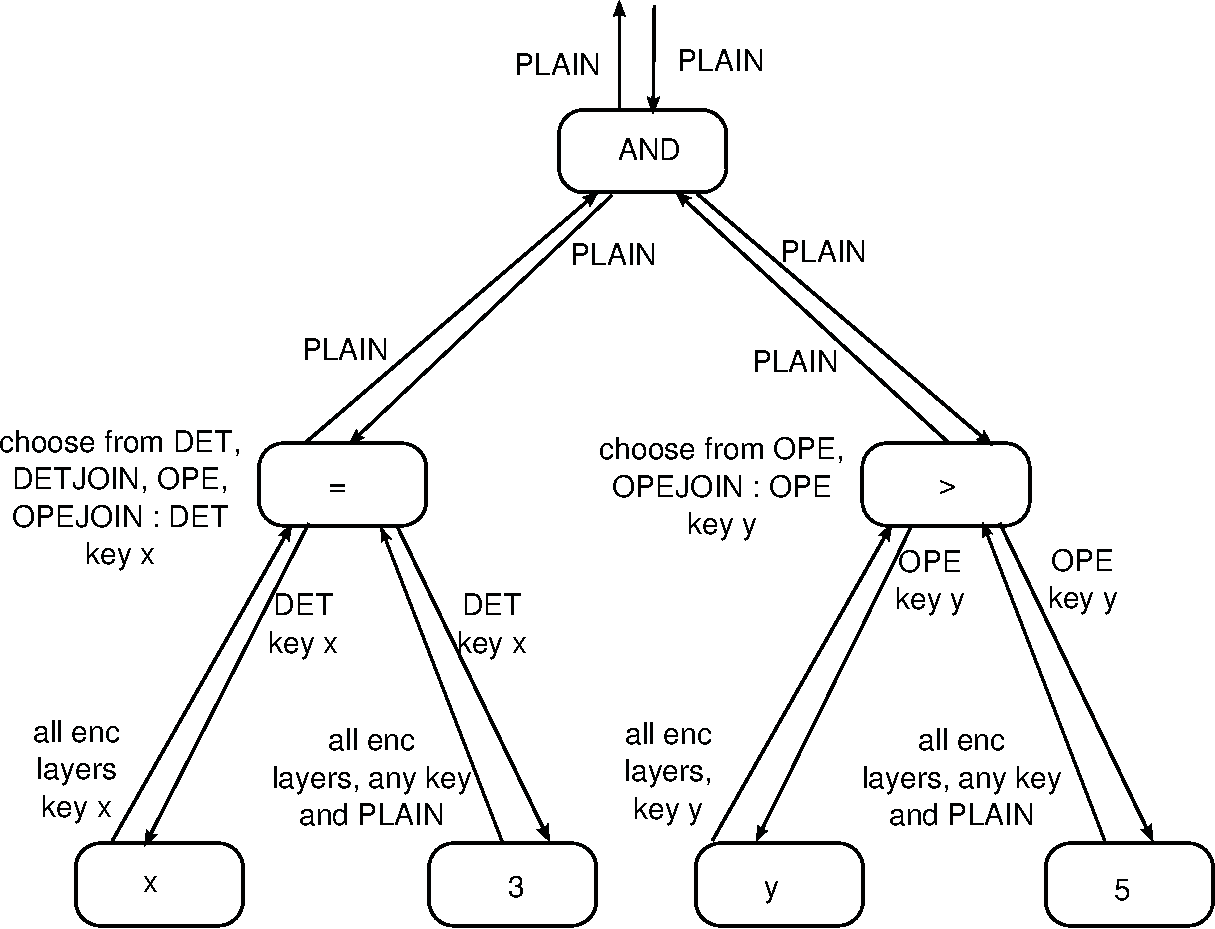
\includegraphics[width=10cm]{fig/gather.pdf}
\caption{Example gather/rewrite for \texttt{x = 3 AND y > 5}. EncSets go up the
  tree in gather and down the tree in rewrite. }
\label{fig:gather}
\end{figure}

\section{Rewrite}

After we computed gather on the entire lex tree, we run rewrite. 

\begin{lstlisting}
 virtual Item *
 do_rewrite_type(Item_field *i, const OLK & constr, Analysis & a) const
\end{lstlisting}

\texttt{do\_rewrite\_type} receives as argument an item $i$ and returns its
rewritten version.

In gather, the top of the lex tree returned an EncSet, from which we pick the
OLK that leaks the least security and provide it as \texttt{constr} argument to
\texttt{do\_rewrite\_type} at the root. 
When \texttt{do\_rewrite\_type} writes for a certain item type, the following
typically happens. First, we consult the \texttt{RewritePlan} for item $i$ (stored in
\texttt{a.itemRewritePlans}). Using this information and \texttt{constr}, we
call  \texttt{do\_rewrite\_type} on the children of node $i$. Finally, we
rewrite $i$, again based on \texttt{constr} and \texttt{do\_rewrite\_type}.

If a rewrite needs to perform onion adjustment, an exception is thrown, the
onions adjusted, and the entire gather/rewrite process restarted.


\bibliographystyle{plain}

\bibliography{internals}




\end{document}

